\apendice{Documentación de usuario}

\section{Introducción}

Este anexo presenta una guía de uso de UBU E-R App desde el punto de vista del usuario final. Su objetivo es explicar cómo acceder a la aplicación y cómo utilizar sus principales funcionalidades para crear, validar, importar, exportar y transformar diagramas Entidad-Relación.

A diferencia de la documentación técnica de programación, este apartado no describe la estructura interna del código ni las decisiones de implementación. El propósito es ofrecer una referencia práctica para manejar la aplicación de forma autónoma, explicando las acciones habituales sobre el lienzo y sobre los elementos del diagrama.

Para facilitar el seguimiento del manual, las acciones se explican mediante un ejemplo sencillo basado en empleados y oficinas. Este ejemplo permite mostrar de forma progresiva la creación de entidades, atributos, claves primarias, relaciones, cardinalidades, validación del diagrama y generación de SQL. El manual no pretende cubrir todas las combinaciones posibles del modelo E/R, sino presentar un flujo representativo de uso de la aplicación.

La aplicación está orientada principalmente a usuarios con conocimientos básicos del modelo Entidad-Relación. Por ello, se asume que el usuario conoce los conceptos generales de entidad, atributo, relación, cardinalidad y clave primaria, aunque la propia interfaz incorpora mensajes de ayuda, acciones contextuales y validaciones para facilitar el trabajo con el editor.

\section{Requisitos de usuario}

Para utilizar la aplicación, el usuario debe cumplir los siguientes requisitos básicos:

\begin{itemize}
    \item Disponer de un navegador web actualizado. Durante el desarrollo se ha trabajado y probado principalmente con navegadores basados en Chromium y con Firefox.

    \item Tener conexión a Internet si se utiliza la versión desplegada de la aplicación.

    \item Contar con conocimientos básicos sobre diagramas Entidad-Relación y sobre su transformación al modelo relacional.

    \item Disponer de un dispositivo con pantalla y ratón, panel táctil o mecanismo equivalente que permita interactuar con el lienzo gráfico.
\end{itemize}

Aunque la aplicación ofrece ayuda contextual y mensajes de validación, es recomendable que el usuario conozca previamente los elementos principales del modelo E/R. En particular, resulta útil entender la diferencia entre entidades fuertes y débiles, atributos simples, compuestos o multivaluados, relaciones binarias y ternarias, cardinalidades y claves primarias.

\section{Instalación}

La forma principal de utilizar UBU E-R App es mediante la versión desplegada de la aplicación. En este caso no es necesario instalar nada en el equipo del usuario, ya que la aplicación se ejecuta directamente desde el navegador web:

\begin{center}
\href{https://draw-entity-relation-opal.vercel.app/}{Aplicación web desplegada}
\end{center}

Para utilizar esta versión basta con abrir el enlace anterior en un navegador actualizado. La aplicación no requiere autenticación, registro de usuario ni configuración previa. El trabajo realizado se conserva en el almacenamiento local del navegador y también puede guardarse mediante la exportación del diagrama en formato JSON.

De forma alternativa, el proyecto puede ejecutarse localmente. Esta opción está orientada principalmente a revisión técnica, pruebas o continuación del desarrollo, por lo que se describe con más detalle en el manual del programador. De manera resumida, se requiere tener instalados Node.js y npm, clonar el repositorio, instalar las dependencias y arrancar el servidor de desarrollo:

\begin{verbatim}
git clone <url-del-repositorio>
cd <directorio-del-proyecto>
npm install
npm start
\end{verbatim}

Tras ejecutar estos comandos, la aplicación estará disponible normalmente en la dirección local indicada por la terminal, habitualmente:

\begin{verbatim}
http://localhost:3000
\end{verbatim}

También puede generarse una versión preparada para producción mediante:

\begin{verbatim}
npm run build
\end{verbatim}

Esta ejecución local no es necesaria para el uso habitual de la aplicación, pero permite revisar el funcionamiento del proyecto fuera del despliegue web.

\section{Manual del usuario}

En esta sección se describe el uso principal de la aplicación mediante un recorrido guiado. El ejemplo utilizado representa una situación sencilla en la que una organización tiene empleados que trabajan en oficinas. A partir de este caso se muestran las operaciones habituales del editor: crear entidades, añadir atributos, configurar relaciones, validar el diagrama, generar SQL y guardar o exportar el trabajo.

\subsection{Pantalla principal}

Al acceder a la aplicación se muestra la pantalla principal del editor. La interfaz está formada por un panel lateral de herramientas y acciones, y un lienzo central donde se construye el diagrama Entidad-Relación.

En la figura se muestra la pantalla principal con las dos entidades iniciales del ejemplo utilizado en el manual.

\imagen{editor_general_anexos}{Pantalla principal de UBU E-R App con las entidades iniciales del ejemplo.}

La zona principal de trabajo es el lienzo. Sobre él se colocan las entidades, atributos, relaciones y otros elementos del modelo. El usuario puede seleccionar los elementos creados para moverlos, modificarlos o aplicar acciones contextuales.

En el panel lateral se encuentran las herramientas de creación, las acciones contextuales y las acciones generales del diagrama. Estas opciones permiten crear nuevos elementos, modificar los elementos seleccionados, validar el modelo, generar SQL, importar o exportar diagramas y acceder a la ayuda de la aplicación.

Cuando no hay ningún elemento seleccionado, la aplicación muestra las acciones generales disponibles. Al seleccionar un elemento del lienzo, el panel lateral se adapta y muestra las acciones que tienen sentido para ese tipo de elemento.

\subsection{Componentes de la interfaz}

La interfaz de la aplicación se organiza en dos zonas principales. Por un lado, el panel lateral agrupa el acceso al cambio de idioma, las herramientas de creación, las acciones contextuales y las acciones generales del diagrama. Por otro lado, el lienzo de edición ocupa la zona central y permite construir visualmente el modelo Entidad-Relación.

\begin{figure}[H]
    \centering
    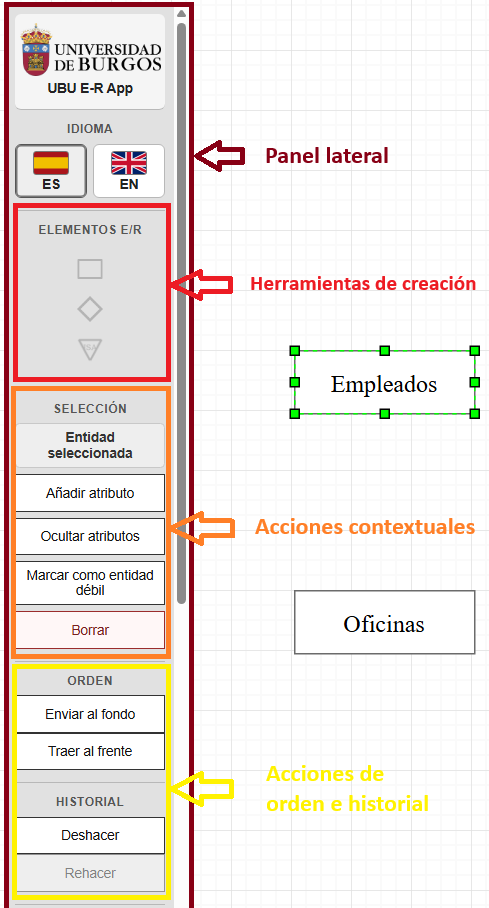
\includegraphics[height=0.66\textheight,keepaspectratio]{img/acciones_contextuales_entidad}
    \caption{Panel lateral con herramientas de creación y acciones contextuales de una entidad seleccionada.}
    \label{fig:acciones_contextuales_entidad}
\end{figure}

Al seleccionar un elemento del lienzo, el panel lateral muestra acciones contextuales asociadas a ese tipo de elemento. En la figura anterior se muestra el caso de una entidad seleccionada, donde aparecen operaciones como añadir atributos, ocultar atributos, marcar la entidad como débil, modificar el orden visual o eliminarla.

Además de las acciones contextuales, la aplicación incorpora acciones generales que afectan al diagrama completo. Estas acciones permiten generar estructuras de ejemplo, comprobar el diagrama, ajustar la vista, generar SQL, exportar o importar diagramas, exportar una imagen del lienzo y reiniciar el trabajo actual.

\begin{figure}[H]
    \centering
    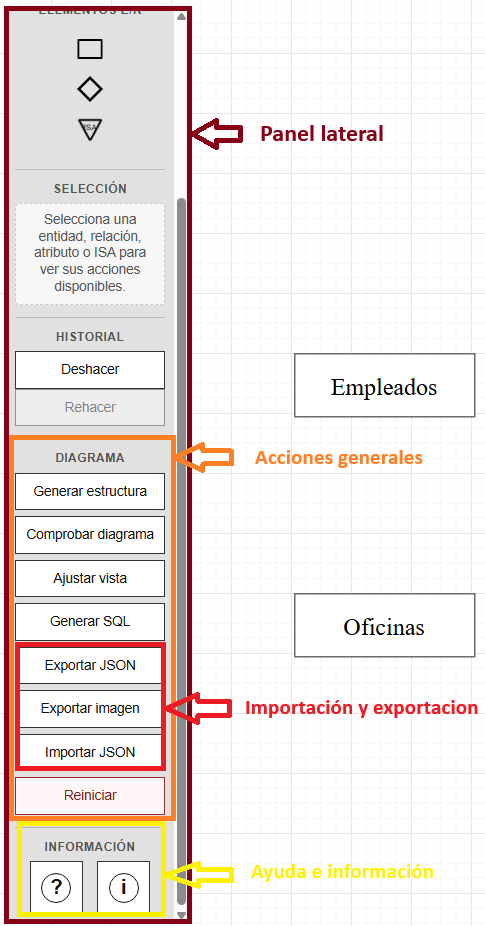
\includegraphics[height=0.66\textheight,keepaspectratio]{img/acciones_generales_diagrama}
    \caption{Panel lateral con acciones generales, importación, exportación y ayuda del editor.}
    \label{fig:acciones_generales_diagrama}
\end{figure}

Esta separación entre acciones contextuales y acciones generales permite que el usuario distinga entre operaciones aplicadas a un elemento concreto y operaciones aplicadas al conjunto del diagrama.

\subsection{Crear un diagrama sencillo}

El ejemplo del manual se basa en dos entidades: \textit{Empleados} y \textit{Oficinas}. La entidad \textit{Empleados} representa a los trabajadores de una organización, mientras que \textit{Oficinas} representa las sedes en las que pueden trabajar.

Para comenzar el diagrama se siguen estos pasos:

\begin{enumerate}
    \item Arrastrar una entidad desde el panel lateral hasta el lienzo.
    \item Cambiar el nombre de la entidad a \textit{Empleados}.
    \item Arrastrar una segunda entidad al lienzo.
    \item Cambiar el nombre de la segunda entidad a \textit{Oficinas}.
    \item Colocar ambas entidades dejando espacio entre ellas para añadir posteriormente la relación.
\end{enumerate}

Una vez creadas las entidades, se añaden sus atributos principales. Para la entidad \textit{Empleados} se pueden definir los atributos \textit{idEmpleado}, \textit{nombre} y \textit{email}. Para la entidad \textit{Oficinas} se pueden definir los atributos \textit{idOficina}, \textit{nombre} y \textit{ciudad}.

Para añadir atributos a una entidad:

\begin{enumerate}
    \item Seleccionar la entidad en el lienzo.
    \item Utilizar la acción contextual para añadir un atributo.
    \item Introducir el nombre del atributo.
    \item Repetir el proceso hasta completar los atributos necesarios.
\end{enumerate}

Después de añadir los atributos, deben marcarse las claves primarias. En este ejemplo, \textit{idEmpleado} identifica a cada empleado e \textit{idOficina} identifica a cada oficina.

Para marcar un atributo como clave primaria:

\begin{enumerate}
    \item Seleccionar el atributo correspondiente.
    \item Utilizar la acción contextual para marcarlo como clave primaria.
    \item Comprobar visualmente que el atributo queda representado como identificador.
\end{enumerate}

\imagen{diagrama_empleados_oficinas}{Entidades \textit{Empleados} y \textit{Oficinas} con sus atributos y claves primarias.}

Este primer paso permite construir la parte básica del modelo antes de incorporar relaciones entre entidades.

\subsection{Crear una relación entre entidades}

Una vez creadas las entidades \textit{Empleados} y \textit{Oficinas}, se añade una relación entre ambas. En el ejemplo se utiliza la relación \textit{Trabaja\_en}, que representa que los empleados trabajan en oficinas.

Para crear la relación:

\begin{enumerate}
    \item Arrastrar una relación desde el panel lateral hasta el lienzo.
    \item Cambiar el nombre de la relación a \textit{Trabaja\_en}.
    \item Seleccionar la relación creada.
    \item Abrir la acción contextual de configuración de participantes.
    \item Seleccionar como participantes las entidades \textit{Empleados} y \textit{Oficinas}.
    \item Confirmar la configuración.
\end{enumerate}

\imagen{configuracion_relacion}{Configuración de los participantes de la relación \textit{Trabaja\_en}.}

La relación todavía no está completa hasta que se indiquen sus cardinalidades. En este ejemplo se quiere representar que una oficina puede tener cero o varios empleados y que cada empleado trabaja en una única oficina. Para ello, se configura la relación con cardinalidad \textit{(0,n)} asociada a \textit{Empleados} y \textit{(1,1)} asociada a \textit{Oficinas}, de acuerdo con la notación utilizada en el editor.

Para configurar las cardinalidades:

\begin{enumerate}
    \item Seleccionar la relación \textit{Trabaja\_en}.
    \item Abrir la acción contextual de cardinalidades.
    \item Definir la cardinalidad correspondiente a cada participante.
    \item Confirmar los cambios.
    \item Revisar visualmente que las cardinalidades aparecen en el diagrama.
\end{enumerate}

\imagen{configuracion_cardinalidades}{Configuración de cardinalidades de la relación \textit{Trabaja\_en}.}

La correcta configuración de participantes y cardinalidades es necesaria para que la aplicación pueda validar el diagrama y transformar posteriormente el modelo E/R al modelo relacional.

\subsection{Validar el diagrama}

Antes de generar el SQL, es recomendable comprobar que el diagrama está completo y no contiene errores básicos. La validación revisa aspectos como la existencia de claves primarias, la configuración de relaciones, la ausencia de nombres repetidos y la definición correcta de cardinalidades.

Para validar el diagrama:

\begin{enumerate}
    \item Revisar que las entidades principales tienen atributos.
    \item Comprobar que cada entidad tiene definida su clave primaria.
    \item Confirmar que las relaciones tienen participantes y cardinalidades.
    \item Pulsar la acción \textit{Comprobar diagrama} en el panel lateral.
    \item Leer el diagnóstico mostrado por la aplicación.
\end{enumerate}

Si el diagrama contiene algún problema, la aplicación muestra un mensaje de validación para indicar qué debe corregirse. Por ejemplo, si la entidad \textit{Empleados} no tuviera atributos o no tuviera clave primaria, el diagnóstico debería señalar ese problema sobre la entidad concreta del ejemplo.

\imagen{dialogo_validacion}{Mensaje de validación asociado a la entidad \textit{Empleados}.}

En la figura se muestra un ejemplo de diagnóstico cuando la entidad \textit{Empleados} no tiene definida una clave primaria. El mensaje identifica el elemento concreto que debe revisarse, lo que facilita corregir el diagrama antes de generar el SQL.

\subsection{Generar SQL}

Cuando el diagrama está validado, la aplicación permite generar un script SQL a partir del modelo E/R construido. En el ejemplo de empleados y oficinas, la generación produce una representación relacional con las tablas, claves primarias y claves ajenas necesarias para reflejar la relación entre ambas entidades.

Para generar el SQL:

\begin{enumerate}
    \item Comprobar previamente el diagrama.
    \item Corregir los errores indicados por la validación, si los hubiera.
    \item Pulsar la acción \textit{Generar SQL}.
    \item Revisar el script mostrado por la aplicación.
    \item Copiar o guardar el resultado si se desea utilizar como referencia.
\end{enumerate}

\imagen{sql_generado}{Script SQL compatible con PostgreSQL generado a partir del ejemplo.}

El SQL generado por la aplicación está orientado a PostgreSQL. La salida incluye sentencias de creación de tablas, claves primarias y claves ajenas derivadas de la transformación relacional del diagrama. No obstante, debe interpretarse como una ayuda académica para comprender la correspondencia entre el modelo E/R y el modelo relacional, no como un generador industrial completo preparado para cubrir todas las decisiones físicas de una base de datos real.

\subsection{Guardar, importar y exportar diagramas}

La aplicación permite guardar y recuperar diagramas mediante ficheros JSON. Esta funcionalidad resulta útil para conservar el trabajo realizado, compartir un diagrama con otra persona o continuar editándolo en otro momento.

Para guardar el diagrama actual:

\begin{enumerate}
    \item Pulsar la acción de exportación JSON.
    \item Guardar el fichero generado en el equipo.
    \item Conservar ese fichero si se desea reabrir posteriormente el diagrama en la aplicación.
\end{enumerate}

El fichero JSON contiene la información necesaria para reconstruir el diagrama, incluyendo sus elementos, configuración y posiciones en el lienzo.

Para importar un diagrama:

\begin{enumerate}
    \item Pulsar la acción de importación JSON.
    \item Seleccionar el fichero que se desea cargar.
    \item Elegir si el contenido importado debe reemplazar el diagrama actual o combinarse con él.
    \item Confirmar la operación.
\end{enumerate}

\imagen{importacion_json}{Importación de un diagrama desde un fichero JSON.}

La opción de reemplazar resulta adecuada cuando se desea abrir un diagrama guardado y trabajar únicamente sobre él. En cambio, la opción de combinar permite añadir los elementos importados al diagrama que ya está abierto.

Además de la exportación JSON, la aplicación permite exportar una representación visual del diagrama. Esta opción genera una imagen del lienzo en formatos como PNG o SVG, pensada para incluir el diagrama en documentos, entregas o material de apoyo. A diferencia del JSON, estos formatos visuales no están pensados para volver a editar el diagrama dentro de la aplicación, sino para obtener una copia gráfica del resultado.

\subsection{Acciones de edición y visualización}

Durante la construcción del diagrama, el usuario puede modificar los elementos creados directamente desde el lienzo. Las acciones disponibles dependen del tipo de elemento seleccionado.

Al seleccionar una entidad, pueden aparecer acciones para añadir atributos, mostrar u ocultar atributos asociados, marcar la entidad como débil, cambiar su orden visual o eliminarla. Al seleccionar un atributo, pueden aparecer acciones para marcarlo como clave primaria, convertirlo en multivaluado, crear subatributos o eliminarlo. Al seleccionar una relación, pueden configurarse sus participantes, cardinalidades y atributos propios cuando proceda.

La aplicación también permite seleccionar varios elementos a la vez. Esta funcionalidad resulta útil cuando el usuario quiere reorganizar una parte del diagrama o eliminar varios elementos en una única operación.

\begin{figure}[H]
    \centering
    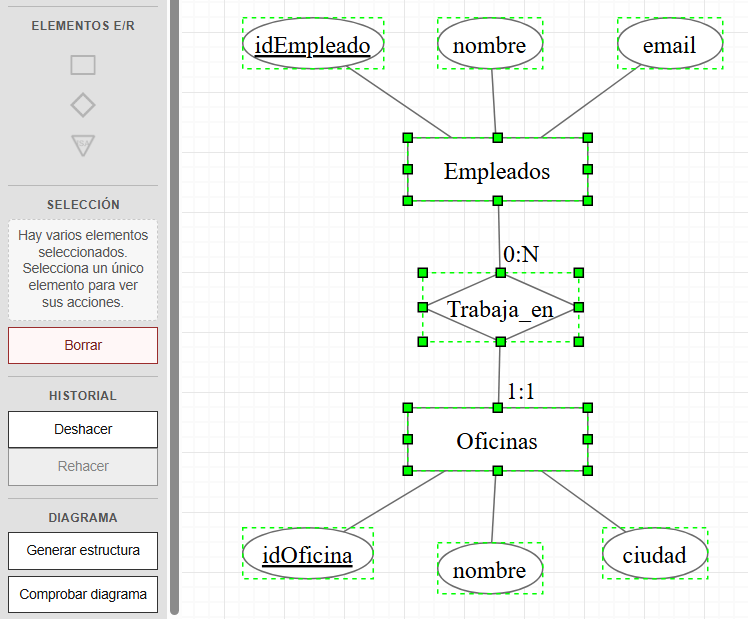
\includegraphics[width=0.82\textwidth,keepaspectratio]{img/seleccion_multiple}
    \caption{Selección múltiple de elementos en el lienzo.}
    \label{fig:seleccion_multiple}
\end{figure}

Cuando existe una selección múltiple, la interfaz evita mostrar acciones individuales que solo tendrían sentido para un tipo concreto de elemento. En su lugar, se mantienen disponibles las operaciones aplicables al conjunto seleccionado, como mover o eliminar los elementos seleccionados.

Entre las acciones generales de visualización también se encuentra el ajuste de vista, que centra y adapta el contenido del lienzo para facilitar la revisión del diagrama completo. Esta opción resulta útil cuando el modelo ha crecido o cuando algunos elementos han quedado alejados de la zona visible.

\subsection{Generar estructuras predefinidas}

Además de crear los elementos de forma manual, la aplicación permite generar estructuras predefinidas de ejemplo. Esta funcionalidad sirve como apoyo para comenzar rápidamente un diagrama sencillo, probar el comportamiento del editor o revisar cómo se representan determinadas combinaciones de elementos.

Para generar una estructura predefinida:

\begin{enumerate}
    \setlength{\itemsep}{0.15em}
    \setlength{\parskip}{0pt}
    \item Seleccionar la acción de generación de estructuras en el panel lateral.
    \item Elegir el tipo de estructura que se desea insertar.
    \item Indicar si la estructura debe reemplazar el diagrama actual o combinarse con el contenido existente.
    \item Confirmar la operación.
\end{enumerate}

\begin{figure}[H]
    \centering
    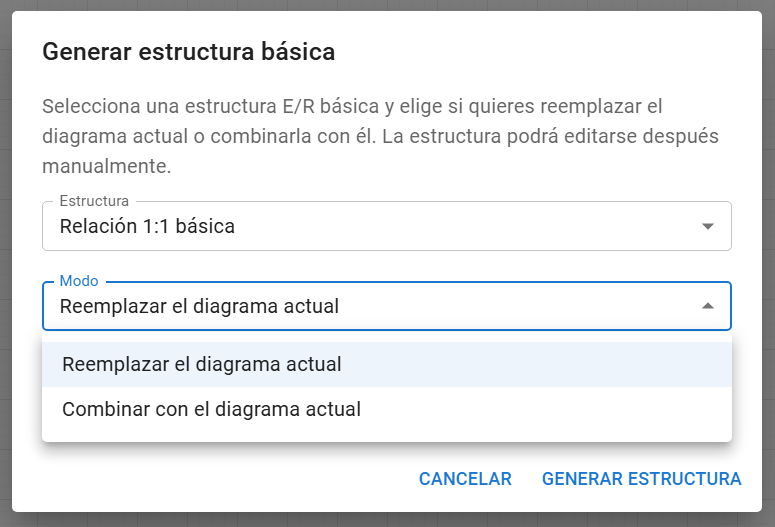
\includegraphics[width=0.72\textwidth,keepaspectratio]{img/generacion_estructuras}
    \caption{Generación de estructuras predefinidas en el editor.}
    \label{fig:generacion_estructuras}
\end{figure}

La opción de reemplazar resulta adecuada cuando se quiere empezar desde una estructura limpia. La opción de combinar permite añadir la estructura generada al diagrama que ya se está editando. En este segundo caso, el usuario debe revisar visualmente el resultado para comprobar que la combinación mantiene el sentido del modelo.

Esta funcionalidad no sustituye al modelado manual del diagrama, sino que actúa como una ayuda para crear ejemplos, realizar pruebas o acelerar la construcción inicial de un modelo sencillo.

\subsection{Uso de elementos avanzados}

UBU E-R App incorpora soporte para algunos elementos avanzados del modelo Entidad-Relación dentro del alcance definido en este TFG. Estos elementos permiten construir diagramas más completos, aunque requieren una configuración cuidadosa para que la validación y la generación SQL sean coherentes.

\subsubsection{Entidades débiles}

Para utilizar una entidad débil, el usuario debe crear primero la entidad propietaria y la entidad que dependerá de ella. Después debe marcar la entidad correspondiente como débil, configurar la relación identificadora y definir el discriminante.

El flujo habitual es el siguiente:

\begin{enumerate}
    \item Crear la entidad propietaria.
    \item Crear la entidad que se desea tratar como entidad débil.
    \item Marcar la entidad correspondiente como débil desde sus acciones contextuales.
    \item Configurar la relación identificadora con la entidad propietaria.
    \item Definir el discriminante de la entidad débil.
    \item Validar el diagrama.
\end{enumerate}

Si falta la entidad propietaria, la relación identificadora o el discriminante, la validación informa del problema para que el usuario pueda corregirlo.

\subsubsection{Relaciones ternarias y roles}

Las relaciones ternarias permiten representar interrelaciones en las que participan tres entidades. Para utilizarlas, el usuario debe crear la relación, configurar sus participantes y definir sus cardinalidades.

El flujo habitual es el siguiente:

\begin{enumerate}
    \item Crear las entidades participantes.
    \item Crear la relación en el lienzo.
    \item Abrir la configuración de la relación desde las acciones contextuales.
    \item Seleccionar los tres participantes.
    \item Definir las cardinalidades correspondientes.
    \item Añadir roles cuando una entidad participe más de una vez o cuando sea necesario aclarar el significado de cada participación.
\end{enumerate}

Los roles ayudan a distinguir participaciones ambiguas, especialmente cuando una misma entidad interviene en más de un papel dentro de la relación.

\subsubsection{Jerarquías ISA}

La aplicación permite representar jerarquías ISA sencillas, formadas por una entidad general y una o varias especializaciones. Este soporte es inicial y controlado, por lo que no incluye discriminantes ISA, herencia múltiple real ni restricciones de totalidad, parcialidad, solapamiento o exclusividad.

El flujo habitual es el siguiente:

\begin{enumerate}
    \item Crear la entidad que actuará como generalización.
    \item Crear una o varias entidades especializadas.
    \item Insertar el elemento ISA en el lienzo.
    \item Configurar la entidad general y sus especializaciones mediante las acciones disponibles.
    \item Validar el diagrama para detectar configuraciones incompletas o no soportadas.
\end{enumerate}

En la transformación relacional soportada por la aplicación, la clave de la entidad general se hereda en las especializaciones. Por ello, las entidades especializadas no deben definir una clave propia independiente.

\subsection{Ayuda, idioma e información del proyecto}

La aplicación incluye varias acciones de apoyo pensadas para facilitar su uso y proporcionar información adicional al usuario.

El selector de idioma permite alternar entre español e inglés. Al cambiar el idioma, la interfaz actualiza sus textos principales, incluyendo botones, mensajes de ayuda y diagnósticos mostrados al usuario.

La acción de ayuda muestra una guía breve sobre el funcionamiento general de la aplicación. Esta guía sirve como referencia rápida para recordar cómo crear elementos, utilizar las acciones contextuales, validar el diagrama o generar SQL.

La opción de información del proyecto muestra datos generales sobre la aplicación, incluyendo su nombre, autoría, créditos, tecnologías utilizadas, referencia al proyecto original y licencia de la versión actual.

\imagen{about_aplicacion}{Información general de UBU E-R App.}

Estas acciones complementan el flujo principal de edición y contribuyen a que la aplicación sea más comprensible para usuarios que acceden por primera vez al editor.

\subsection{Flujo de trabajo recomendado}

Aunque la aplicación permite editar el diagrama de forma flexible, se recomienda seguir un flujo de trabajo ordenado para reducir errores y facilitar la generación posterior del SQL.

De forma resumida, el flujo habitual de uso es el siguiente:

\begin{enumerate}
    \item Crear las entidades principales del modelo.
    \item Añadir atributos y definir claves primarias.
    \item Incorporar relaciones entre entidades.
    \item Configurar participantes y cardinalidades.
    \item Añadir elementos adicionales, como entidades débiles, atributos de relación, relaciones ternarias o estructuras ISA, cuando proceda.
    \item Comprobar el diagrama mediante la validación.
    \item Generar y revisar el SQL compatible con PostgreSQL.
    \item Exportar el diagrama en JSON si se quiere conservar para futuras ediciones.
    \item Exportar el diagrama como imagen si se quiere incluir en documentación o material de apoyo.
\end{enumerate}

Este flujo no es obligatorio, pero ayuda a mantener el diagrama coherente y facilita que la transformación relacional refleje correctamente el modelo diseñado.
